\chapter{Background}
\label{ch:background}

\section{Difficulty of CMA-ES}

Being an outstanding local optimizer, CMA-ES performs well on figuring out solutions in a restrict region.
This property, however, leads CMA-ES to a premature convergence when the search space grows largely.

we can first take a look at the figure~\ref{fig:localExample} to illustrate the described hazard.
\begin{figure}[h]
\begin{center}
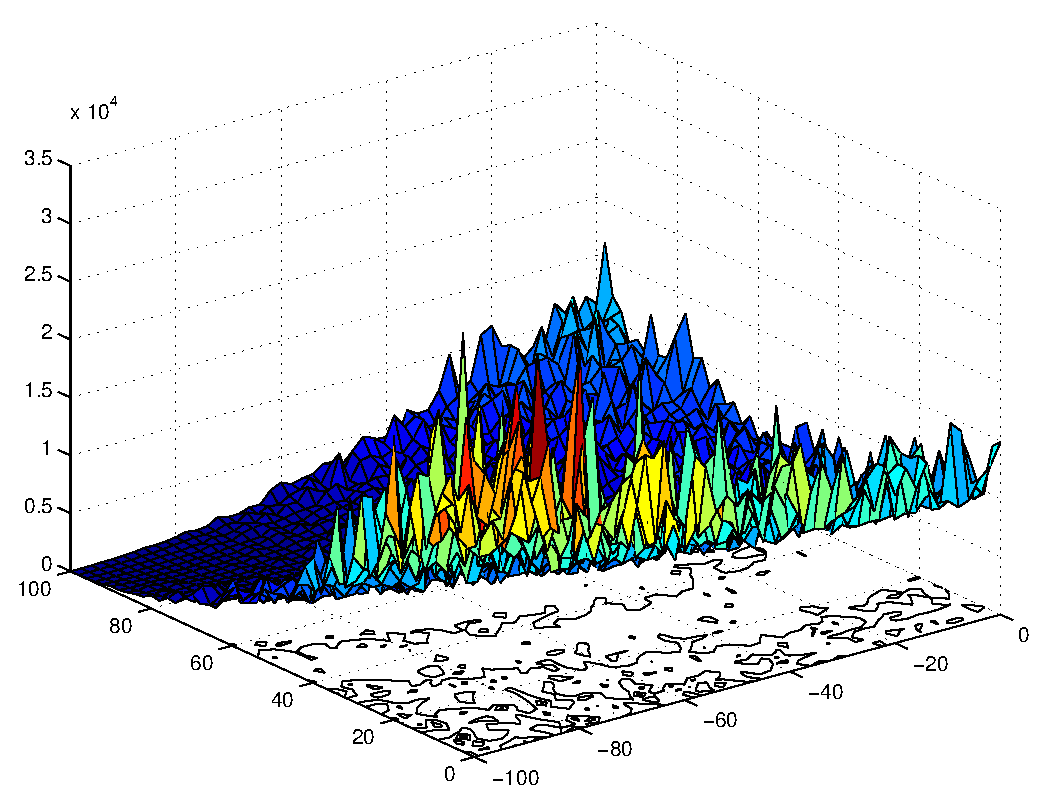
\includegraphics[scale = 0.5]{2Dproblem3DMap.eps}
\caption{Example for local optima}
\label{fig:localExample}
\end{center}
\end{figure}
This is an example for fitness landscape of 2-D function, and the goal is to minimize the function value.
From the shown distribution of fitness we can imagine that there should be a number of valley, which we refer to as local optimum, in real-valued optimization problems.
With a small population, it is impossible to fetch global optimum unless the initial population are just sampled right around the best valley.
Due to the rugged property of real-valued optimization problems, CMA-ES being a good local optimizer is just easily trapped in one of the local optima.

Generally in evolution algorithm, the most popular solution to the hazard is increasing the population in order to observe a high diversity.
CMA-ES, however, obtains no benefits from the method.
The reason can be distinguished by the mechanism of sampling.
If a huge population is applied and sampled uniformly, it can only be said that the mean vector comes closer to the central of the search space.
However, the population size affects only the initial position of the mean vector $m$.
As the routine starting to execute, the population size turns to be useless because it is $\mu$ and $\lambda$ that controls the size of evolution.
At the second generation, $m$ is updated by the weighted mean of selected solutions, which was affected not only initialed $m$ but initialed step size, initialed covariance matrix, etc.
That is to say, with a huge amount of initial population, the only affected condition is that the expected distance of $m$ and the center of search space becomes shorter. 
The evolution path are then driven towards the region where the fit solutions are in the early stage, and this means the property of diversity we wish to obtained according to a huge population size is not useful under the mechanism.
 


\section{The hypothesis to conquer the difficulty}

The original form of CMA-ES faces the problem described above.
To conquer the difficulty, the first idea comes from that if we are able to roughly estimate the region where the global optimum locates.
Once there is just a small region, CMA-ES is believed to be capable of finding out the optimum inside.
The technique of estimation 
